\chapter{Rešerše}
\label{0-reserse}

Pro přiblížení se k oficiálně publikovaným tarifním pásmům byly potřeba využít algoritmy
digitální kartografie. Tarifní pásma jsou publikována mimo jiné jako shapefile 
\footnote{formát vektorového datového úložiště Esri pro ukládání umístění,
tvaru a atributů geografických prvků \cite{shapefile}}, který obsahuje
vektorové prostorových dat ve formě polygonových prvků. K této podobě bylo potřeba přistoupit
za pomocí některých vybraných algoritmů.

\subsubsection{Triangulace}
\label{triangulace}

K vytvoření linií mezi jednotlivými zastávkami slouží takzvaná triangulace, 
která vytvoří troj\-úhelníky mezi body tak, že uvnitř těchto trojúhelníků  
už neleží žádné body a každý trojúhelník má vždy společnou jednu hranu. 

%% ML: Postup triangulace (?)
Triangulace se používají jak v kartografii, tak v \zk{GIS}, v Dálkovém průzkumu země (\zk{DPZ}),
počítačové grafice, při analýze vlastností a struktury materiálů, plánování pohybu robotů
nebo při modelování přírodních jevů. \cite{bayer-delaunay}

Existuje více druhů triangulací, které využívají vždy jinou metodu konstrukce
a mají rozdílný výpočetní stupeň složitosti. 

%% ML: nazvy dejte napr. do kurzivy, aby se vizualne dolisila od textu
\textit{Hladová (Greedy) triangulace} se snaží vytvářet trojúhelníky s nejkratšími stranami,
které nesplňují žádnou speciální geometrickou podmínku. Její realizace je jednoduchá,
avšak důsledkem toho jsou často tvarově nepěkné nebo nevhodné trojúhelníky. Má velkou výpočetní
složitost \(O(n^3)\), lze optimalizovat na \(O(n^2 \log(n))\). V kartografii se
kvůli její složitosti často nepoužívá. \cite{vanicek}

\begin{figure}[H] \centering
    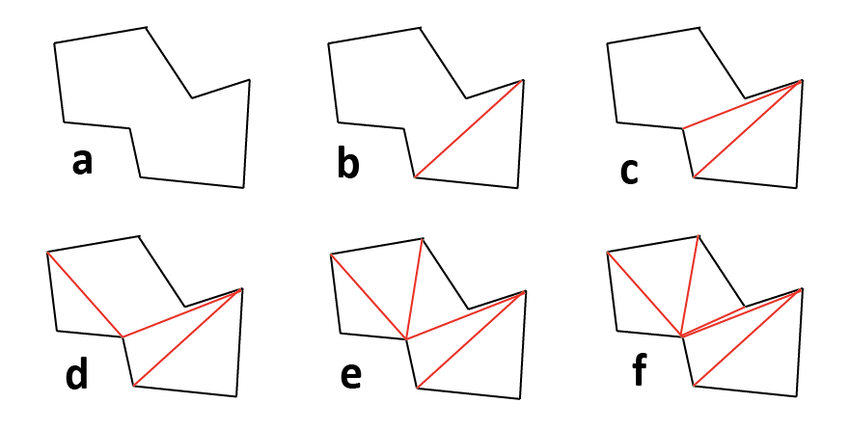
\includegraphics[width=400pt]{./pictures/triangulace-greedy.png}
    \caption[Ilustrace Greedy triangulace]{Ilustrace Greedy triangulace \cite{triangulace-greedy}}
	\label{fig:triangulace-greedy}              
\end{figure}

Další triangulací je tzv. \textit{Delaunay triangulace}, která je nejčastěji používaná.
\textit{Delaunay triangulací} se rozumí vytváření liniových spojnic bodů mezi jednotlivými body, které jsou si nejblíže,
za pomocí opsaných kružnic. \textit{Delaunay triangulace} má několik vlastností. Jednou z nich je například,
že uvnitř kružnice k opsané libovolnému trojúhelníku neleží žádný jiný bod.
Zároveň \textit{Delaunay triangulace} je jednoznačná, pokud žádné čtyři body neleží na kružnici.
Na rozdíl od \textit{Greedy triangulace} nehodnotí kritérium délky hran. Díky maximalizaci minimálních
úhlů vytváří takové trojúhelníky, které se nejvíc blíží k rovnostranným trojúhelníkům, 
což znamená, že se snaží eliminovat trojúhelníky, které jsou ostroúhlé.

Pro výtváření konstrukce \textit{Delaunay triangulace} jsou k dispozici různé algoritmy: lokální prohazování, 
inkrementální konstrukce, inkrementální vkládání, rozděl a panuj nebo sweep line. \cite{bayer-delaunay}

\begin{figure}[H] \centering
    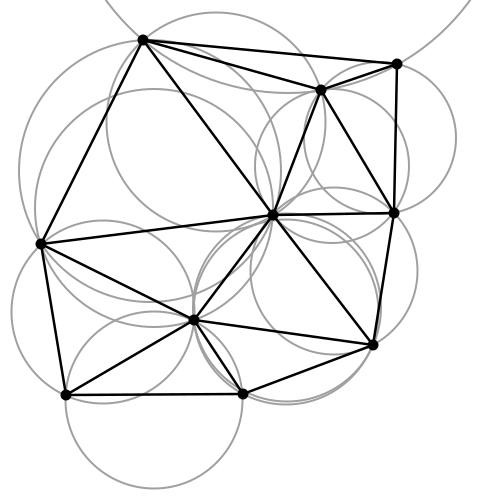
\includegraphics[width=280pt]{./pictures/triangulace-delaunay.png}
    \caption[Ilustrace Delaunay triangulace]{Ilustrace Delaunay triangulace \cite{triangulace-delaunay}}
	\label{fig:triangulace-delaunay}              
\end{figure}

Poté existuje \textit{triangulace s minimální hmotností} (anglicky \textit{Minimum Weight Triangulation}, zkráceně MWT),
%%% ML: Na zaklade ceho je "nejlepsi" ???
která má minimální celkovou délku hran. MWT je nejlepší triangulace pro interpolaci trojrozměrných oblastí,
tudíž se pro tvorbu 2D tarifních pásem úplně nehodí.

\subsubsection{Konvexní obálka}
\label{konv_obalka}

Pro vytváření hranic polygonů je konvexní obálka jedna z možností, co použít. Konvexní obálka (anglicky Convex hull)
je nejmenší konvexní množinou, pokud spoj\-nice  libovolných dvou prvků leží zcela uvnitř této množiny.
Je to jedna z nejpoužívanějších geometrických struktur, která je většinou používána jako první odhad
prostorového tvaru.

Konstrukce konvexní obálky se nejčastěji provádějí metodami: Jarvis Scan, Graham Scan, QuickHull nebo
rozděl a panuj. Konvexní obálku lze vytvářet i pomocí \textit{Delaunay triangulace}, kdy se po jejím dokončení
spojí všechny trojúhelníky.

\begin{figure}[H] \centering
    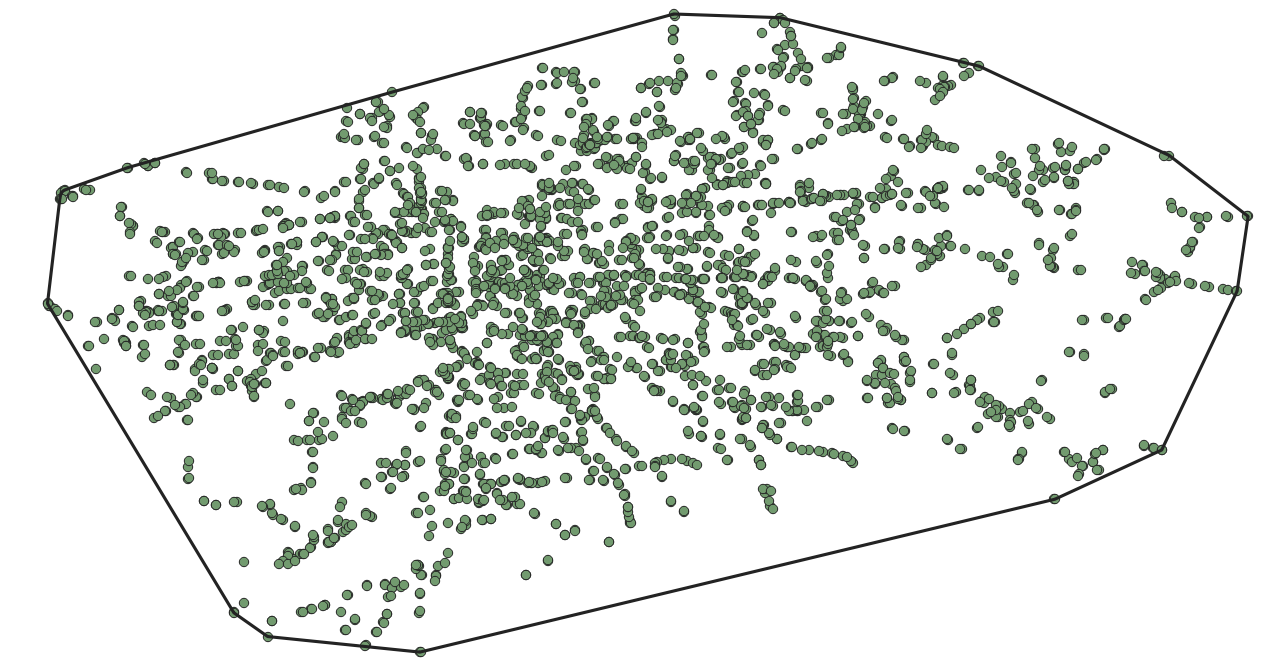
\includegraphics[width=400pt]{./pictures/convexHull.png}
    \caption[Konvexní obálka]{Konvexní obálka}
	\label{fig:convexHull}              
\end{figure}

\subsubsection{Konkávní obálka}
\label{konk_obalka}
 
Oproti konvexní obálce je konkávní obálka pro tvorbu složitější. Není znám přesný postup,
jak tento problém řešit, ale existují různé aproximace, které se k tomu chtějí přiblížit.
První aproximace je pomocí \textit{Delaunay triangulace}, kde se vytvoří trojúhelníky, vznikne
konvexní obálka a pak se odebírají trojúhelníky s nevhodnými vlastnostmi. Typicky mají příliš ostrý nebo tupý
úhel, hraniční hodnota vlastností se může zvolit.
Předpokladem pro úspěšně fungování je to, že množina bodů má konstantní
prostorovou hustotu bodů.

Další aproximací je pomocí \textit{alpha-shapes}, kde se volí parametr alpha. Představme si obrovskou masu zmrzliny,
která tvoří prostor \(R^3\) a obsahující body jako \uv{tvrdé} kousky čokolády. Pomocí jedné z těchto 
zmrzlinových lžiček ve tvaru koule vyřezáme všechny části zmrzlinového bloku, na které se dostaneme,
aniž bychom narazili na kousky čokolády, a tím dokonce vydlabeme otvory uvnitř 
(např. části nedosažitelné pouhým pohybem lžíce z venku). Nakonec skončíme s 
(ne nutně konvexním) objektem ohraničeným oblouky a body. Pokud nyní narovnáme všechny 
\uv{kulaté} plochy na trojúhelníky a úsečky, máme intuitivní popis toho, co se nazývá alpha-shape. \cite{alpha-shapes}

Další strategií je kompromisní definice mezi alpha-shapes a konkávní obálkou, tzv. alpha-concave
hull. 

\begin{figure}[H] \centering
    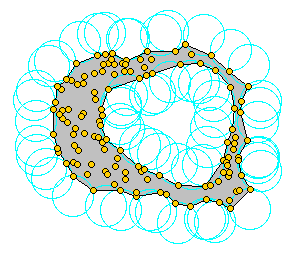
\includegraphics[width=296pt]{./pictures/alphashape.png}
    \caption[Konvkávní obálka pomocí alpha-shapes]{Konvkávní obálka pomocí alpha-shapes \cite{alpha-shapes-picture}}
	\label{fig:alpha-shapes-picture}              
\end{figure} 

%% ML: vetsinu pojmu mate cesky (sklonovane), https://cs.wikipedia.org/wiki/Voron%C3%A9ho_diagram
\subsubsection{Voronoi diagram}

Tarifní pásma zasahují hranicí tam, kde nejsou žádné zastávky. Pro takové vyplnění plochy
mezi zastávkami a pro místa, kde zastávky nejsou (většinou na krajích zón) není triangulace, konvexní nebo konkávní 
obálka úplně vhodná. Pro takový problém bylo další myšlenkou použít teselaci, což je vyplnění roviny pomocí jednoho
nebo více geometrických útvarů vzájemně spojených, bez překryvů a mezer. Triangulace, konvexní nebo konkávní 
obálka se mohou hodit při dalších krocích výpočtu.

Nejpoužívanější teselací v oblastí GIS je \textit{Voronoi diagram}, někdy nazývána Voroné\-ho teselace, Voroného dekompozice,
Thiessenovy polygony nebo Dirichletova teselace, což je způsob rozkladu 
metrického prostoru určený vzdálenostmi k dané nespojité množině bodů v prostoru.
V našem případě se bude řešit Voronoi diagram ve 2D prostoru, tedy v rovině.

%% ML: Opakujete v jedne vete "Voronoi diagram", prepiste
Na vstupu je nějaká množina bodů a výstupem je \textit{Voronoi diagram}, 
což představuje takovou množinu buněk, pro které bude platit, že každý bod
\textit{q} náležící množině \textit{V(p\textsubscript{i})} je blíže k bodu
\textit{p\textsubscript{i}} než k jakémukoliv
bodu \textit{p\textsubscript{j}} náležící množině \textit{P}.  \cite{bayer-voronoi}

Pro lepší chápání \textit{Voronoi diagramů} je potřeba si vysvětlit její terminologii.
Vstup\-ní množinu bodů nazýváme generátory, každý bod generuje jednu Voronoi buňku. V 
terminologii GIS se hovoří o tzv. Voronoi polygony. Tyto Voronoi buňky jsou tvořeny hranami,
které spojují dva Voronoi vrcholy. Dohromady tyto Voronoi buňky tvoří Voronoi diagram.  

\begin{figure}[H] \centering
    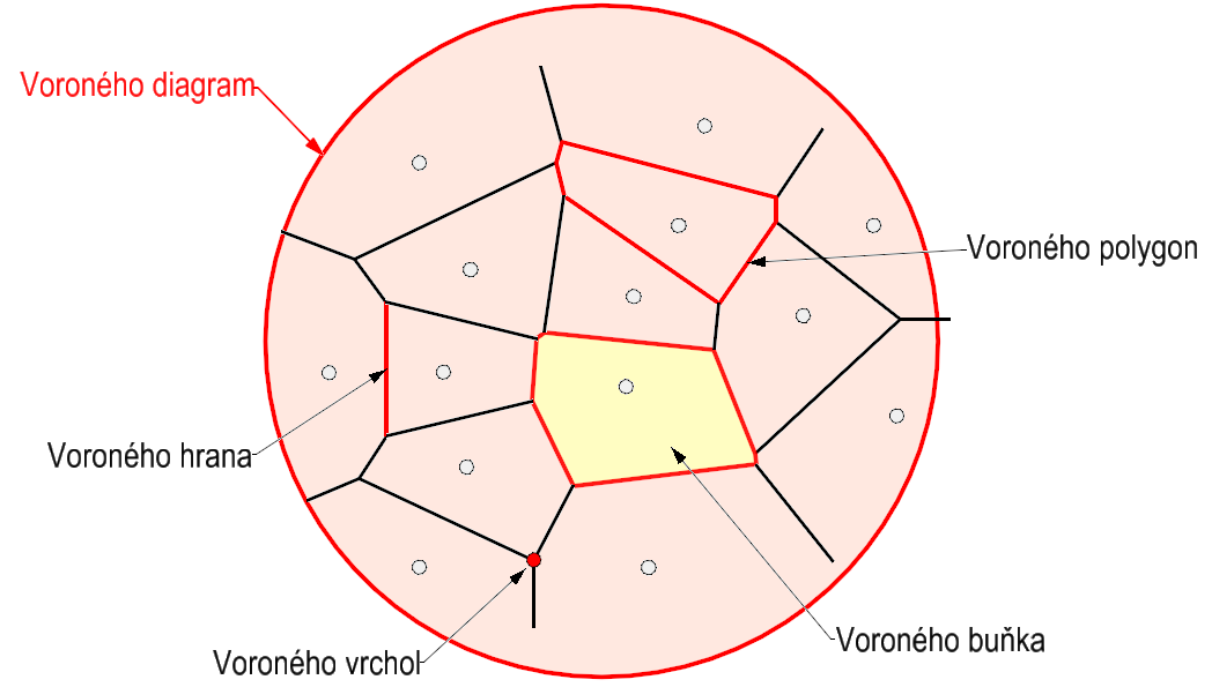
\includegraphics[width=400pt]{./pictures/bayer-voronoi-terminologie.png}
    \caption[Terminologie Voronoi diagramu]{Terminologie Voronoi diagramu \cite{bayer-voronoi}}
	\label{fig:bayer-voronoi-terminologie}              
\end{figure}

\textit{Voronoi diagramy} mají své vlastnosti, které jsou důležité pro jejich tvorbu. V následujících
odrážkách jsou doslovně citována jejich znění z prezentace pana doc. Ing. Tomáše Bayera, Ph.D.

\begin{quote}
\begin{itemize}

\item Voronoi diagram \textit{V(P)} je planárním grafem.
\item Vrchol q Voronoi buňky \textit{\{V(p\textsubscript{i})} je průnikem 3 hran, právě když je \textit{V(P)} nedegenerovaný.
\item Pokud \textit{p\textsubscript{i}} náležící \textit{H(P)}, pak je \textit{V(p\textsubscript{i})}  otevřený. 
\item Pro každý bod \textit{p\textsubscript{i} náležící P} je \textit{V(P)} konvexní. 
\item Bod \textit{p\textsubscript{i}} je nejbližším bodem bodu \textit{p}
jestliže \textit{p} náleží \textit{\{V(p\textsubscript{i})}.
\item Každá strana \textit{q\textsubscript{i}q\textsubscript{j}}, \(i \neq j\),
je sdílena právě dvěma sousedními buňkami \textit{V(p)}. 
\item Bod q je vrcholem \textit{V(p)}, pokud existuje kružnice \textit{k(q,r)} procházející třemi
nebo více generátory \textit{p\textsubscript{i}}, \textit{p\textsubscript{j}},
\textit{p\textsubscript{k}}, a neobsahuje žádný další bod P (spojitost s \textit{DT(P)}). 
\item Kružnici \textit{k(q,r)} označujeme jako největší prázdnou kružnici ze všech prázdných kružnic se středem v bodě \textit{q}. 
\item Průměrné množství Voronoi hran ve Voronoi polygonu nepřekročí hodnotu 6. 
\item Vztah mezi počtem bodů \textit{n}, počtem hran \textit{n\textsubscript{h}}
a počtem trojúhelníků \textit{n\textsubscript{t}} teselace \textit{V(P)}:
\[ n_h \leq 3n-6\]
\[ n_t \leq 2n−5\]
\item Voronoi diagram \textit{V(P)} představuje ortografickou projekci stěn
mnohostěnu tvořeného průsečnicemi všech polorovin \textit{A\textsubscript{i}} do roviny \textit{xy}. 
\item Nechť bod \textit{p\textsubscript{i}\textsuperscript{*}} i představuje
ortografický průmět bodu \textit{p\textsubscript{i}} na povrch paraboloidu daného rovnicí:
\[ z = x^2 + y^2 \]
   
\end{itemize}
\end{quote}

\begin{figure}[H] \centering
    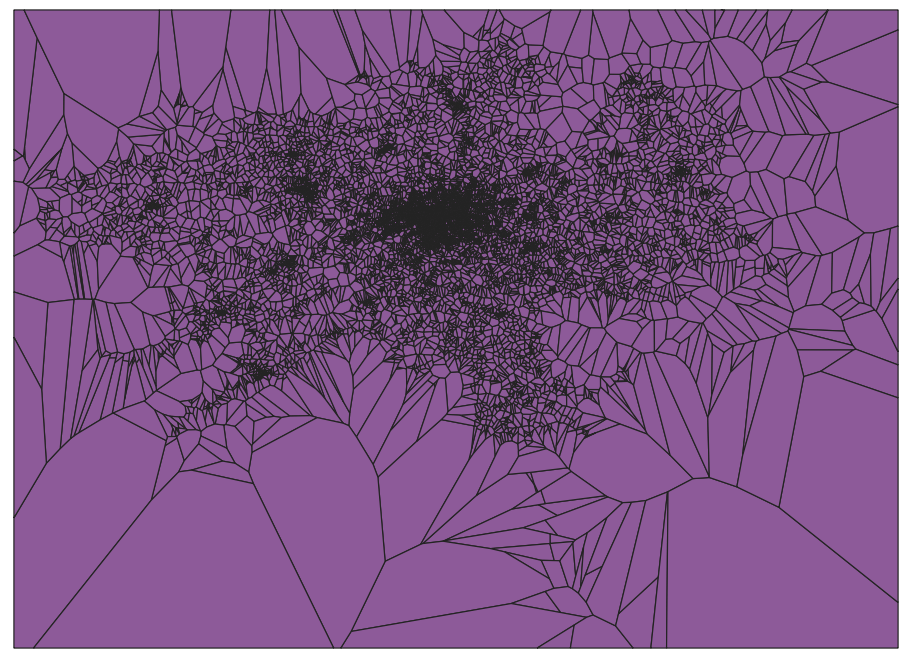
\includegraphics[width=400pt]{./pictures/voronoi.png}
    \caption[Voronoi polygony]{Voronoi polygony}
	\label{fig:voronoi}              
\end{figure}   

\textit{Voronoi diagram} má spojitost s \textit{Delaunay triangulací}. Hraniční vstupní body
\textit{Voronoi diagramu} po spojení \textit{Delaunay triangulací} tvoří konvexní obálku.
Středy kružnic opsaných trojúhelníků \textit{Delaunay triangulace} představují uzlové body
\textit{Voronoi diagramu}.

Pro konstrukci \textit{Voronoi diagramu} existují různé metody. Konstrukce lze v praxi tvořit přímo nebo nepřímo.
Pro přímou konstrukci jsou tu metody inkrementální konstrukce, sweep line algoritmus a
rozděl a panuj. Nepřímá konstrukce je vytvářena přes \textit{Delaunay triangulaci} skrz spojení středů
kružnic opsaných trojúhelníků a bývá nejpoužívanější. 

%% ML: postovni problem ???
Využití Voronoi diagramů v oblasti GIS je široké. Například tzv. poštovní problém
pomáhá při návrhu nových supermarketů, stanic MHD či polohy nových nemocnic.
Mezi další využití patří například převod bodových údajů na plošné
nebo klasifikace dat. \cite{bayer-voronoi}

\subsubsection{Generalizace a zjemnění}
\label{generalizace_zjemneni}

Pro přiblížení se výsledku k graficky estetičtější verzi je potřeba hranice polygonů
generalizovat. Následně se hranice zjemní. K tomu existuje mnoho algoritmů, ale bude zde uvedeno
jen několik vhodných a nejpoužívanějších.

Jedním z nich je generalizační algoritmus \textit{Douglas-Peucker}. Algoritmus rekurzivně rozděluje čáru.
Zpočátku jsou uvedeny všechny body mezi prvním a posledním bodem. Automaticky označí první a poslední bod,
který se má zachovat. Poté najde bod, který je nejvzdálenější od úsečky s prvním a posledním bodem 
jako koncovými body. Tento bod je zjevně nejvzdálenější na křivce od přibližné úsečky mezi koncovými body. 
Pokud je bod blíže k úsečce, než volitelný parametr epsilon, mohou být všechny body, které nejsou aktuálně označeny jako zachované,
zahozeny, aniž by rozměr zjednodušené křivky byl menší než parametr epsilon. Pokud je nejvzdálenější bod od úsečky větší než parametr epsilon od aproximace,
musí být tento bod zachován. Algoritmus rekurzivně volá sebe samotného s prvním bodem a nejvzdálenějším bodem 
a poté nejvzdálenějším bodem a posledním bodem, který zahrnuje nejvzdálenější bod označený jako ponechaný.
%% ML: proc "nejlepsi"?
Tento algoritmus je jeden z nejlepších generalizačních algoritmů a je velmi často
implementován v GIS softwarech. \cite{bayer-douglas}

\begin{figure}[H] \centering
    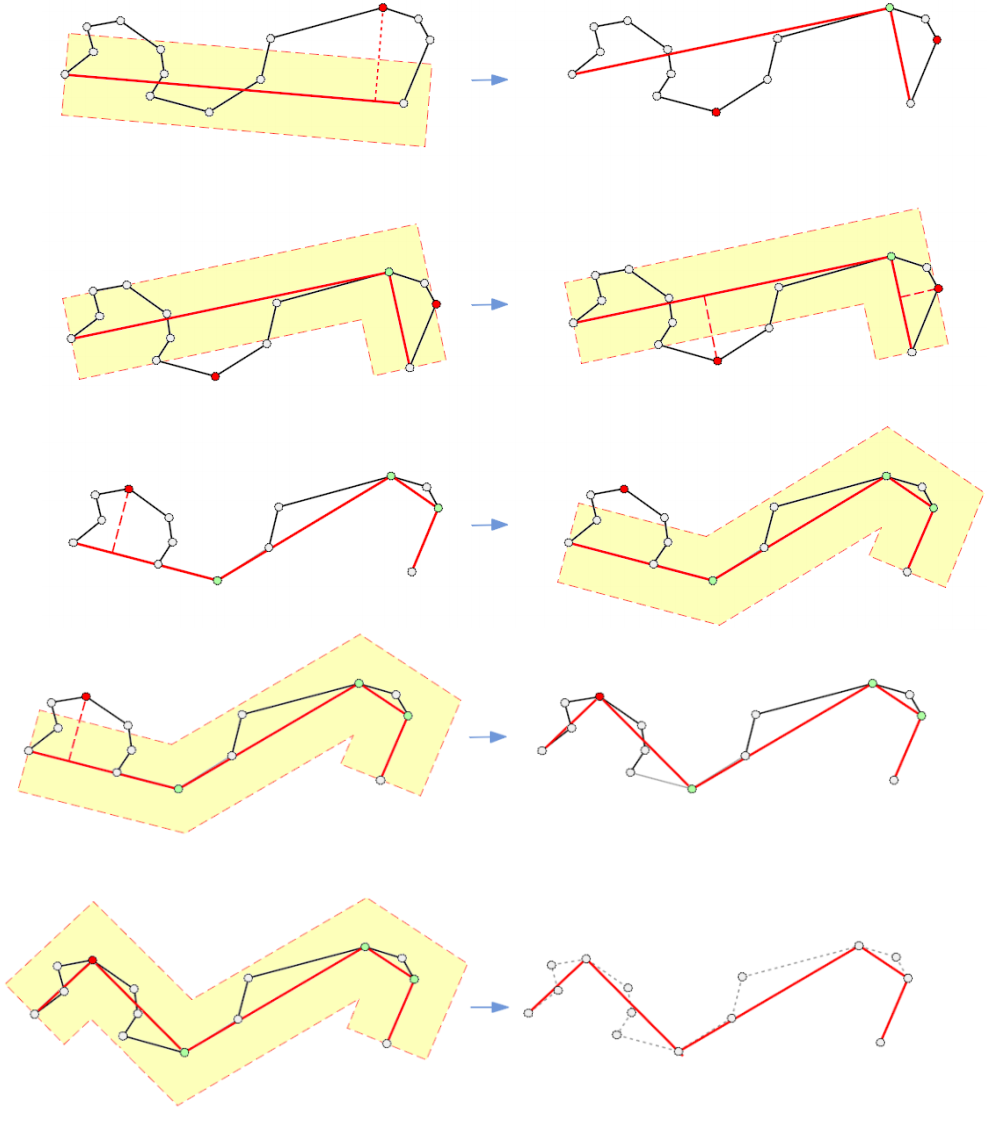
\includegraphics[width=400pt]{./pictures/douglas.png}
    \caption[Znázornění algoritmu \uv{Douglas-Peucker}]{Znázornění algoritmu \uv{Douglas-Peucker} \cite{bayer-douglas}}
	\label{fig:douglas}              
\end{figure} 

Dalším algoritmem je zjemňovací/vyhlazovací algoritmus \textit{Polynomická aproximace metodou Exponenciálního jádra}
(anglicky textit{Polynomial Approximation with Exponential Kernel}, zkráceně PAEK).
Tento algoritmus vyvinula společnost Esri pro nástroj Smooth Line a je jejím soukromým vlastnictvím.
Ačkoliv se zdá být ideální, tak není použitelný pro jiné platformy kvůli nezveřejněnému algoritmu.

Podobným algoritmem jako PAEK je algoritmus \textit{Chaikinův}. 
Chaikin (autor algoritmu, po kterém je i algoritmus pojmenován) využil fixních poměrů na odříznutí rohů, takže byly všechny rozřezány stejně. 
Při matematickém zápisu postupuje Chaikinova metoda následovně: Dostaneme kontrolní polygon 
\textit{\{P\textsubscript{0}, P\textsubscript{1}, ..., P\textsubscript{n}\}},
tento kontrolní polygon vylepšíme vygenerováním nové posloupnosti řídících bodů 
\[ \{Q_0, R_0, Q_1, R_1, ...,  Q_{n−1}, R_{n−1}\} \]                                    
kde každou novou dvojici bodů Q\textsubscript{i}, R\textsubscript{i} je třeba brát v poměru \(\frac{1}{4}\)
a \(\frac{3}{4}\) mezi koncovými body segmentu čáry \(\overline{P\textsubscript{i}P\textsubscript{i+1}}\).
\[Q_i = \frac{3}{4}P_i + \frac{1}{4}P_{i+1}\]
\[R_i = \frac{1}{4}P_i + \frac{3}{4}P_{i+1}\]
Tyto 2 nové body lze považovat za nový řídicí polygon - vylepšení původního řídícího polygonu. 
Tento postup lze pro tentýž úsek opakovat, čímž vznikne vyhlazená čára. \cite{chaikin} 

\begin{figure}[H] \centering
    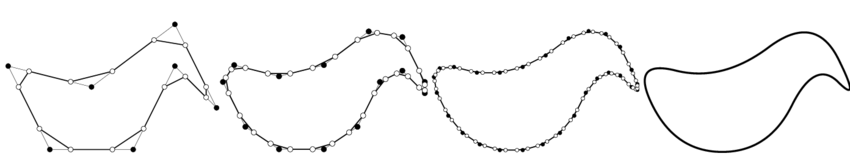
\includegraphics[width=400pt]{./pictures/chaiken.png}
    \caption[Znázornění Chaikinova algoritmu]{Znázornění Chaikinova algoritmu \cite{bayer-douglas}}
	\label{fig:chaiken}              
\end{figure} 